%% Preambel
\documentclass[conference,compsoc,final,a4paper]{IEEEtran}
\usepackage[utf8]{inputenx}

%% Bitte legen Sie hier den Titel und den Autor der Arbeit fest
\newcommand{\autoren}[0]{NACHNAME, VORNAME}
\newcommand{\dokumententitel}[0]{Vorlage für eine Seminararbeit}

% Pakete einbinden, die benötigt werden
\usepackage{scrpage2}
\usepackage{graphicx}             % Bilder einbinden
\usepackage{xcolor}               % Color support
\usepackage{amsmath}              % Matheamtische Formeln
\usepackage{amsfonts}             % Mathematische Zeichensätze
\usepackage{amssymb}              % Mathematische Symbole
\usepackage{float}                % Fließende Objekte (Tabellen, Grafiken etc.)
\usepackage{booktabs}             % Korrekter Tabellensatz
\usepackage[printonlyused]{acronym}  % Abkürzungsverzeichnis [nur verwendete Abkürzugen]
\usepackage{makeidx}              % Sachregister
\usepackage{listings}             % Source Code listings
\usepackage{listingsutf8}         % Listings in UTF8
\usepackage[hang,font={sf,footnotesize},labelfont={footnotesize,bf}]{caption} % Beschriftungen
\usepackage[scaled]{helvet}       % Schrift Helvetia laden
\usepackage[sf,bf,small]{titlesec} % Einstellungen für Überschriften
\usepackage[absolute]{textpos}	  % Absolute Textpositionen (für Deckblatt)
\usepackage{calc}                 % Berechnung von Positionen
\usepackage{blindtext}            % Blindtexte
\usepackage[bottom=40mm,left=35mm,right=35mm,top=30mm]{geometry} % Ränder ändern
\usepackage{setspace}             % Abstände korrigieren
\usepackage{ifthen}               % Logische Bedingungen mit ifthenelse
\usepackage{scrhack}              % Get rid of tocbasic warnings
%\usepackage[pagebackref=false]{hyperref}  % Hyperlinks
%\usepackage{rotating}             % Seiten drehen

%\setlength{\bibitemsep}{1em}     % Abstand zwischen den Literaturangaben
%\setlength{\bibhang}{2em}        % Einzug nach jeweils erster Zeile

% Farben definieren
\definecolor{linkblue}{RGB}{0, 0, 100}
\definecolor{linkblack}{RGB}{0, 0, 0}
\definecolor{comment}{RGB}{63, 127, 95}
\definecolor{darkgreen}{RGB}{14, 144, 102}
\definecolor{darkblue}{RGB}{0,0,168}
\definecolor{darkred}{RGB}{128,0,0}
\definecolor{javadoccomment}{RGB}{0,0,240}

% Einstellungen für das Hyperlink-Paket
\hypersetup{
    colorlinks=true,      % Farbige links verwenden       
%    allcolors=linkblue,
    linktoc=all,          % Links im Inhaltsverzeichnis
    linkcolor=linkblack,  % Querverweise
    citecolor=linkblack,  % Literaturangaben
	filecolor=linkblack,  % Dateilinks
	urlcolor=linkblack    % URLs
}

% Einstellungen für Quelltexte
\lstset{     
      xleftmargin=0.2cm,     
      basicstyle=\footnotesize\ttfamily,
      keywordstyle=\color{darkgreen},
      identifierstyle=\color{darkblue},
      commentstyle=\color{comment}, 
      stringstyle=\color{darkred}, 
      tabsize=2,
      lineskip={2pt},
      columns=flexible,
      inputencoding=utf8,
      captionpos=b,
      breakautoindent=true,
	  breakindent=2em,
	  breaklines=true,
	  prebreak=,
	  postbreak=,
      numbers=none,
      numberstyle=\tiny,
      showspaces=false,      % Keine Leerzeichensymbole
      showtabs=false,        % Keine Tabsymbole
      showstringspaces=false,% Leerzeichen in Strings
      morecomment=[s][\color{javadoccomment}]{/**}{*/},
      literate={Ö}{{\"O}}1 {Ä}{{\"A}}1 {Ü}{{\"U}}1 {ß}{{\ss}}2 {ü}{{\"u}}1 {ä}{{\"a}}1 {ö}{{\"o}}1
}

\urlstyle{same}

\titlespacing{\paragraph}{0pt}{1ex}{2.0ex}
\titlespacing{\subsubsection}{0pt}{3ex}{0.0ex}
\titlespacing{\subsection}{0pt}{4ex}{0.2ex}
\titlespacing{\section}{0pt}{7ex}{1ex}
\titleformat*{\subsubsection}{\sffamily\itshape\bfseries\small}
\titleformat*{\paragraph}{\sffamily\bfseries\small}


% Einstellungen für Überschriften
\renewcommand*{\chapterformat}{%
  \Large\chapapp~\thechapter   % Große Schrift
  \vspace{0.3cm}               % Abstand zum Titel des Kapitels
}

% Abstände für die Überschriften setzen

% In der Kopfzeile nur die kurze Kapitelbezeichnung (ohne Kapitel davor)
\renewcommand*\chaptermarkformat{\thechapter\autodot\enskip}
\automark[chapter]{chapter}

% Einstellungen für Schriftarten
\setkomafont{pagehead}{\normalfont\sffamily}
\setkomafont{pagenumber}{\normalfont\sffamily}
\setkomafont{paragraph}{\sffamily\bfseries\small}
\setkomafont{subsubsection}{\sffamily\itshape\bfseries\small}
\addtokomafont{footnote}{\footnotesize}
\setkomafont{chapter}{\LARGE\selectfont\bfseries}

% Wichtige Abstände
\setlength{\parskip}{0.2cm}  % 2mm Abstand zwischen zwei Absätzen
\setlength{\parindent}{0mm}  % Absätze nicht einziehen
\clubpenalty = 10000         % Keine "Schusterjungen"
\widowpenalty = 10000        % Keine "Hurenkinder"
\displaywidowpenalty = 10000 % Keine "Hurenkinder"
\renewcommand{\footnotesize}{\fontsize{9}{10}\selectfont} % Größe der Fußnoten
\setlength{\footnotesep}{8pt} % Abstand zwischen den Fußnoten

% Index erzeugen
\makeindex

% Einfacher Font-Wechsel über dieses Makro
\newcommand{\changefont}[3]{
\fontfamily{#1} \fontseries{#2} \fontshape{#3} \selectfont}

% Eigenes Makro für Bilder
\newcommand{\bild}[3]{
\begin{figure}[h]
  \centering
  \includegraphics[width=#2]{#1}
  \caption{#3}
  \label{#1}
\end{figure}}

% Wo liegt Sourcecode?
\newcommand{\srcloc}{src/}

% Wo sind die Bilder?
\graphicspath{{bilder/}}

% Makros für typographisch korrekte Abkürzungen
\newcommand{\zb}[0]{z.\,B.\ }
\newcommand{\dahe}[0]{d.\,h.\ }
\newcommand{\ua}[0]{u.\,a.\ }

% Flags für Veröffentlichung und Sperrvermerk
\newboolean{hsmapublizieren}
\newboolean{hsmasperrvermerk}
 % Weitere Einstellungen aus einer anderen Datei lesen

% Eigentliches Dokument beginnt hier
% ----------------------------------------------------------------------------------------------------------

% Kurze Zusammenfassung des Dokuments
\begin{abstract}
% a quick summary or overview of the entire paper 
Outsourcing work is a well known by companies. Software crowdsourcing has a lot of potential to become a major technology in software development. It provides motivations as well as barriers to newcomers and companies. This paper is a systematic literature review. It explains different methods and types of software crowdsourcing. Also it reveals barriers faced by newcomers as well as it show the motivation, from a contributer and from a company view, to take part in an software crowdsourcing / open source software project / FLOSS...   The study provides insights for tool designers, managers and researchers, who want to improve the overall amount and quality of contributing in their projects.
%OTCs nicht vergessen
\end{abstract}

\tableofcontents

% Abschnitte mit \section und Unterabschnitte mit \subsection
\section{Introduction}
Software Crowdsourcing had a huge popularity rise in the last few years, even it exits for a very long time. For community projects, such as Linux or Firefox, it is a well known and existing dependant technique. Without the crowd such projects, e.g. elementary OS, Apache and many more would not be possible. With the rise of software crowdsourcing many people try out crowdsourcing. Before somebody can contribute to an project there are several barriers, which specially newcomers has to overcome. Similiar to software crowdsourcing there are other techniques to get results from the crowd. Those technique are; Free Libre Open Source Software (FLOSS), Free Open Source Software (FOSS) and Open Source Software (OSS). Due to those techniques are all very similiar to software crowdsourcing, all of them are included in the search for barriers newcomers are facing before they successful contribute in such an project. 
%was passiert im welchen abschnitt

\section{Research Method}
To find relevant scientific papers i used search engines, 'GoogleScholar', 'IEEE Xplore', 'ACM Digital Library and 'Springer Link''. Moreover, I focused mainly on researches that are not older than 2016(really?!?), because there were not many papers focusing on the barriers newcomer has to overcome I also selected some older researches. Many reasearches I found did focus on other topics, such as .....
In the end I was able to find ..... papers, where I could use ..... of them. Also I found some literature research papers, which I used to find new papers as well as to match the results of the literature research.

\section{State of the art}
\begin{itemize}
\item Patterns for tearing down contribution barriers to FLOSS projects\cite{Wolff-Marting2013}
	\subitem onion model
\item Cloud-Based Software Crowdsourcing\cite{Tsai2014}
\item Crowdsourcing in Software Engineering: Models, Motivations, and Challenges\cite{LaToza2016}
\item The Economic Motivation of Open Source Software: Stakeholder Perspectives\cite{Riehle2007}
	\subitem community vs commercial
\item Understanding the Impressions, Motivations, and Barriers of One Time Code Contributors to FLOSS Projects: A Survey\cite{Lee2017}
	\subitem Successful FLOSS projects must attract and retain these peripheral developers so they can provide more significant code 					contributions.\cite{Lee2017, Steinmacher2015c}
\item Understanding and Supporting the Choice of an Appropriate Task to Start with in Open Source Software Communities \cite{Steinmacher2015c}
\end{itemize}

Nowadays crowdsourcing can be found in a lot of different areas as the system gets more an more popular. Due to the popularity of crowdsourcing it is no incident that you will find a variety of crowdsourcing platforms, e.g. Idea Bounty, CrowdSpring, 99Designs, TopCoder and many more. Due to the high use of the word it is not possible to coherently classify the term 'crowdsourcing'[1]. As Enrique Estellés-Arolas and Fernando González-Ladrón-de-Guevara in the article 'Towards an integrated crowdsourcing definition'\cite{Estelles-Arolas2012} wrote: 
\begin{quote}
The name crowdsourcing is formed from two words: crowd, making reference to the people who participate in the initiatives; and sourcing, which refers to a number of procurement practices aimed at finding, evaluating and engaging suppliers of goods and services.
\end{quote}

%The different models of Crowdsourcing (competetive vs collaborative)
\subsection{Crowdsourcing models}
During the literature review I found four different types of crowdsourcing models.
Within those four models there are two major ways of software crowdsourcing. The competetive method, which had a incredible increase during the last years. The oldest method is the collaborative, which has its roots in the software crowdsourcing and is still a huge factor if or if not crowdsourced projects are successfull.\newline
The first model ist the competetive, also called commercial, model. In this model the collaborator are contestants to eachother\cite{LaToza2016, Riehle2007}. A natural motivation in this model is to compete against each other and the winner will get a reward of the company. With those two motivations it is no wonder that this model gained a lot of attention in software development. The most popular platform for this model is TopCoder (www.topcoder.com) with over one million people in the community and over seven thousand challanges per year. 
An old model is the 'Peer Production', it is also called to be the community version of SW CS \cite{LaToza2016, Riehle2007}.'Peer Production' is an open source procedure which consists of software projects where the community contributes to their favorite project. There is a huge amount of these community open source projects nowdays. Some of the most known are Linux, Firefox, Apache and Atom. Those projects are great example how the crowd can create a great product. Also this model depents that a lot of people contribute to the project. Like the onion model of free libre open source software (FLOSS) projects the onion model for this crowdsourcing would look similiar. At the core there would be the innovation leaders, those who lead the project. Around them there would be the key contributors, those contributors who work constanly on the project. Those contributors who are just active sometimes, e.g. to fix bugs, are at the outside of the onion model.
Another model is called 'Microtasking'\cite{LaToza2016}. In this model the tasks will split up to several small task. With this procedure there will be a lot of small tasks. Without much time needed to complete one task, many contributors are up to do the task. With this redundancy there will be also some differencies in the solutions. Due to those solutions the requester can select the for him best suited solution. 
A similiar to the previous model is the 'Economic model'\cite{Tsai2014}. The goal of this model is also to maximize the contributions.
The companies are creating strategies to include the crowd. Also, the winner, sometimes also the best three solutions, will receive a reward for his contribution.

%Level 1-4
\subsection{Levels of Crowdsourcing}
The ideas of this subsection were received by the article 'Cloud-based Software Crowdsourcing (Dagstuhl Seminar 13362)'\cite{Huhns2013} written by Huns et al. Due to it was the only paper which described the different levels of crowdsourcing, the ideas will be from this article.\newline
As well there are different method of crowdsourcing there are also different level's. Those levels describe how many contributors work on the contribution as well as how large the task is and how much time the contributors have. Those level's are called 'Level 1' up to 'Level 4', where the first level is describes the individual developer. In this level the commiters have clear tasks, which they have to solve within a few moths. Also, the individuals developers as well as the projects can be ranked.
The second level uses small teams with up to ten people per team. Those teams have up to one year time, depending on the project, to develop their solution for the given task. Also it allows that the developers will get feedback and thoughts from the stakeholders and the community during the developing process. 
The next larger level has teams of more than 10 and up to 100 people and a development time of up to two years. Due to this large time span and the larger teams the crowdsourcing platforms for 'Level 3' crowdsourcing need to have an automated cross-verification and is not suited for commercial crowdsourcing, as well as the largest level. With this technique the platform will automatically check if the requirements are met or not.
The largest level has international factors. The developers, from several countries, develop a large and flexible system. Due to the international factors, those projects has to overcome additional barriers before they can succeed. Those barriers are social-cultural barriers, which will be explained in Section X.



\section{Motivation for software crowdsourcing}
As humans we have two types of motivation. One is the 'intrinsic motivation' and the other one is the 'extrinsic motivation'. Intrinsic Motivation describes the motivation of doing a task for inborn satisfaction\cite{Ryan2000}. Regarding to software crowdsourcing this could be to contribute with reasons like; fun and enjoyment, technical learning, altruism. The oponent of the intrinsic motivation is the extrinsic motivation. Extrinsic motivation play always a role, if the person gets something afterwards to do the task \cite{Ryan2000}.Examples therefor are the career status, reputation, fame, community identification. All of the motivations showed in this section can be defined as instrinsic or extrinsic motivation. Also, in the table \ref{tbl:CntribMoti} you will see that there a slightly more intrinsic motivations than extrinsic motivations from a contributors view. As the subsection "Contributer Perspectives" shows, the amount of both motivation types is similiar. This similiarity is important, because to much of one motivation type can have negative effects on the other type \cite{Hossain2012a}. From a stakeholder views there are only extrinsic goals, as shown in table \ref{tbl:StkhldrMoti}. For companies the similarity of both motivatinos does not count, because the main goal of a company is to get something in return for their work.

%companies
\subsection{Stakeholder Perspectives}
The perspectives for the stakeholders were found in the following papers;
\begin{itemize}
	\item Riehle; The Economic Motivation of Open Source Software: Stakeholder Perspectives\cite{Riehle2007}
	\item LaToza and van der Hoek; Crowdsourcing in Software Engineering: Models, Motivations, and Challenges\cite{LaToza2016}
	\item Hossain; Crowdsourcing: Activities, incentives and users' motivations to participate\cite{Hossain2012}
	\item Tsai et al.; Cloud-Based Software Crowdsourcing\cite{Tsai2014}
\end{itemize}
As a stakeholder views, there are in depth reasons why you should consider investing in the open source market. The companies, which are using the open source market, do not sell the product. More likely, they sell the provision, maintenance and the support for the product. Another motivation is; the companies consider more the opinions of the crowd and let them choose the task to work so. By doing so, more people of the crowd will contribute and also they will find more qualitive solutions to their task. Due to the last two points, the customers will trust your company and the product more. With this in the knowledge the company will have less marketing costs. Also, the number of customers will increase rapidly. The companies can hire and fire employees more easily, because there is an large pool of people who fit to the companie or did already worked on the project. Moreover, it is easier to find and employ specialists, due to every project has its 'core worker'. Those core worker are worker, who are specialists in the projects and also work a long time on it. So the core worker have a lot of knowledge and it is also shown that they lead innovations in the projects\cite{Hossain2012, XY}. As a result of finding an employing specialists those specialists can develop more innovative products. With the diversity of the crowd, companies will get alternative solutions. When a company start to enter the open source software field, they will have less time until the next innovative idea comes up. Also, they will have variable costs. It will be easier to share information and they will find an increase in the development speed. The increase in the development speed is found due to the crowd, as they overtake parts of the development. By spending a longer time on the open source market, your customers will become more loyal and the companies will find less risks by launching a new product. Also, the companies will have a increase of the quality of their software. This is a result of the trust by the customers that the company provises, maintain and support their product for a longer time. All those motivations are listed in the table \ref{tbl:StkhldrMoti}.


\begin{table*}
\centering
%\caption{Stakeholder motivations to use software crowdsourcing}
\renewcommand{\arraystretch}{1.5}
	\begin{tabular}{lrrr} %p{4.5cm}p{1cm}p{1cm}p{1cm} - 
		\textbf{Motivation} & \textbf{Motivation type} & \textbf{Found X times} & \textbf{Papers} \\
		
		\multicolumn{4}{l}{\textbf{Extrinsic Motivation}} \\
		
		the company will have less marketing costs & Extrinsic & 2 & \cite{Hossain2012, Tsai2014}\\

		it is easier to find and employ specialists & Extrinsic & 2 & \cite{LaToza2016, Tsai2014}\\
		
		specialists can develop more innovative products & Extrinsic & 2 & \cite{Hossain2012, Tsai2014} \\
		
		companies will get alternative solutions & Extrinsic & 2 & \cite{LaToza2016, Tsai2014}\\
		
		the company sell the provision, maintenance and the support for the product & Extrinsic & 1 & \cite{Riehle2007} \\
		
		the company find more qualitive solutions to their task & Extrinsic & 1 & \cite{LaToza2016}\\
		
		the number of customers will increase rapidly & Extrinsic & 1 & \cite{Hossain2012} \\
		
		the companies can hire and fire employees more easily & Extrinsic & 1 & \cite{Riehle2007} \\
		
		the company will have less time until the next innovative idea comes up & Extrinsic & 1 & \cite{Hossain2012}\\
		
		the company will have variable costs & Extrinsic & 1 & \cite{LaToza2016}\\
		
		the customers will become more loyal & Extrinsic & 1 & \cite{Hossain2012} \\
		
		the companies will find less risks by launching a new product & Extrinsic & 1 & \cite{Hossain2012}\\
		
		the companies will have a increase of the quality of their software & Extrinsic & X & XY
		
		

	\end{tabular}
	\label{tbl:StkhldrMoti}
\end{table*}


%contributors
\subsection{Contributor Perspectives}
The motivations for this subsection were found in the following papers;
\begin{itemize}
	\item Hannebauer et al.; An Exploratory Study of Contribution Barriers Experienced by Newcomers to Open Source Software Projects\cite{Hannebauer2014}
	\item Hannebauer and Gruhn; On the Relationship Between Newcomer Motivations and Contribution Barriers in Open Source Projects\cite{Hannebauer2017}
	\item Lee et al.; Understanding the Impressions, Motivations, and Barriers of One Time Code Contributors to FLOSS Projects: A Survey\cite{Lee2017}
	\item LaToza and van der Hoek; Crowdsourcing in Software Engineering: Models, Motivations, and Challenges\cite{LaToza2016}
	\item Hossain; Users' motivation to participate in online crowdsourcing platforms\cite{Hossain2012a}
\end{itemize}
A more detailed view and who wrote about which paper will be shown in figure XY.\newline
The motivations for the contributors were listed in several papers. The most named motivation is; improvement of programming skills or learn a new technology. I combined those two motivations because the goal of both is to improve yourself, no matter it is by increasing the developing skills or by learning a complete new developing language. Close to this motivation is that contributors want to learn about the project technologies. The second most motivation I found, is the reason that the contributors need a modification for their own project. Similiar to this motivation I found also that a motivation is to make the project interoperable with one's own products. As often as the motivation before, contributors mentioned also that they enjoy programming. Similar to the contributors enjoy programming there are also contributors who enjoy the intellecutal challenge. Some contributors mentioned also that they want to give something back to the community. Close to the last motivation, to consult FLOSS projects was also found. The belief in the idea of open source projects were also named as motivation. Also evaluating a project was found as a motivation to contribute and to give feedback to the project community. Try out open source software projects and to join a community was also mentioned as motivation. By submitting patches, satisfaction will derive from working in a project and with the community. Also, that the changes will be reviewed by others is also a motivation to contribute. A missing feature is also called to be a motivation. To gain the respect of the community was found bei Hannebauer. Personal visibility and similiar to it reputation were also revelead to motivate contributors. Some contributors maybe get paid to contribute, others may get a reward by submitting. The last motivation I could find is that the contributors will have only to contribute once. They will not have to rebuild their patch for the next version of the project again. As well as the stakeholder motivations, those motivations will be divded into intrinsic and extrinsic motivation and listet in table \ref{tbl:CntribMoti}. With this table you will get a good overview of the contributor motivations.

\begin{table*}
\centering
\caption{Motivations to contribute to a software crowdsourcing project}
\renewcommand{\arraystretch}{1.5} %die Zeilenabstände um 50% vergrößern
	\begin{tabular}{lrrr} %p{4.5cm}p{1cm}p{1cm}p{1cm} - 
		\textbf{Motivation} & \textbf{Motivation type} & \textbf{Found X times} & \textbf{Papers} \\
		
		\multicolumn{4}{l}{\textbf{Intrinsic Motivation}} \\
		
		improvement of programming skills or learn a new technology & Intrinsic & 4 & \cite{Hannebauer2014,Hannebauer2017,Lee2017,LaToza2016} \\
		
		enjoy programming & Intrinsic & 3 & \cite{Hannebauer2017, Hossain2012a, LaToza2016} \\
		
		want to give something back to the community & Intrinsic & 3 & \cite{Hannebauer2014, Hossain2012a, LaToza2016} \\
		
		want to learn about project technologies & Intrinsic & 1 & \cite{Hannebauer2014} \\
		
		enjoy the intellectual challenge & Intrinsic & 1 & \cite{Hannebauer2014} \\
		
		to consult FLOSS projects & Intrinsic & 1 & \cite{Hannebauer2014} \\
		
		The belief in the idea of open source projects & Intrinsic & 1 & \cite{Hannebauer2017} \\
		
		evaluating a project & Intrinsic & 1 & \cite{Hannebauer2014} \\
		
		try out open source software projects & Intrinsic & 1 & \cite{Hannebauer2017} \\
		
		to join a community & Intrinsic & 1 & \cite{Hannebauer2017} \\
		
		satisfaction will derive from working in a project and with the community & Intrinsic & 1 & \cite{Hannebauer2014} \\
		
		the contributors will have only to contribute once & Intrinsic & 1 & \cite{xy}\\
		
		
		\multicolumn{4}{l}{\textbf{Extrinsic Motivation}} \\
		
		need a modification for their own project & Extrinsic & 3 & \cite{Hannebauer2014,Hannebauer2017,Lee2017} \\
				
		personal visibility and reputation & Extrinsic & 2 & \cite{Hannebauer2014, Hossain2012a} \\		
		
		make the project interoperable with one's own products & Extrinsic & 1 & \cite{Hannebauer2014} \\
		
		the changes will be reviewed by others & Extrinsic & 1 & \cite{Hannebauer2014} \\
		
		gain respect of the community & Extrinsic & 1 & \cite{Hannebauer2014} \\
		
		get a reward or paid to contribute & Extrinsic & 1 & \cite{Lee2017} \\
	\end{tabular}
	\label{tbl:CntribMoti}
\end{table*}






\section{The process of joining a OSS project}
\begin{itemize}
\item  Newcomers lurk on mailing lists, read previous discussions, and review public information to learn about people, ongoing activities, history and current status of the community. Lurking appears to be an essential part of the joining process, as newcomers acquire the social and technical knowledge expected of participants [31, 36, 42, 43]. [Beyond Pretty Pictures Examining The Benefits of Code Visu...]
\item After acquiring some knowledge about the project and
its norms, newcomers start interacting with other
members by joining discussions and take part in
peripheral activities such as reporting or fixing bugs. [Beyond Pretty Pictures Examining The Benefits of Code Visu...]
\item Observations of newcomers show that successful
joiners do not typically start by introducing themselves
or expressing their interest in contributing. Instead,
they participate in ongoing technical discussions about
existing problems [14, 42]. [Beyond Pretty Pictures Examining The Benefits of Code Visu...]
\item Their initial messages are
not limited to suggesting technical solutions for
problems but often include code, suggesting a high
degree of technical knowledge and skills is required [Beyond Pretty Pictures Examining The Benefits of Code Visu...]
\end{itemize}


\section{barriers faced by newcomers}
\begin{itemize}
\item Understanding the Impressions, Motivations, and Barriers of One Time Code Contributors to FLOSS Projects: A Survey\cite{Lee2017}
\item Understanding and Supporting the Choice of an Appropriate Task to Start with in Open Source Software Communities\cite{Steinmacher2015c}
\item An Exploratory Study of Contribution Barriers Experienced by Newcomers to Open Source Software Projects\cite{Hannebauer2014}
\item Barriers Faced by Newcomers to Software-Crowdsourcing Projects\cite{Zanatta2017}
\item On the Relationship Between Newcomer Motivations and Contribution Barriers in Open Source Projects\cite{Hannebauer2017}
\item The Good, the Bad and the Ugly: An Onboard Journey in Software Crowdsourcing Competitive Model\cite{Machado2017}
\item The Hard Life of Open Source Software Project Newcomers\cite{Steinmacher2014b}
\item Why do newcomers abandon open source software projects?\cite{Steinmacher2013}
\item Patterns for tearing down contribution barriers to FLOSS projects\cite{Wolff-Marting2013}
\item Labeling relevant skills in tasks: Can the crowd help?\cite{Leano2016}

\item SLR's
	\subitem A systematic literature review on the barriers faced by newcomers to open source software projects\cite{Steinmacher2015a}
	\subitem Barriers Faced by Newcomers to Open Source Projects: A Systematic Review\cite{Steinmacher2014}
	\subitem Overcoming Open Source Project Entry Barriers with a Portal for Newcomers\cite{Steinmacher2016}
	\subitem Preliminary Empirical Identification of Barriers Faced by Newcomers to Open Source Software Projects\cite{Steinmacher2014a}
	\subitem Social Barriers Faced by Newcomers Placing Their First Contribution in Open Source Software Projects\cite{Steinmacher2015b}
\end{itemize}

There are many barriers newcomers face by contributing for the first time. Some barriers are larger and other are smaller. I found in my literature review 56 barriers, why newcomer may not contribute to an crowdsourcing project. I conducted barriers, which have semantically the same meaning. Also, I subdivided the barriers into X categories. This categorization and conducting the barriers will provide a more simplified and a more meaningfull statement. It seems like that newcomers have the most problems to rebuild the system where the bug was in. This barrier I found most in the review
\begin{figure*}
	\center
	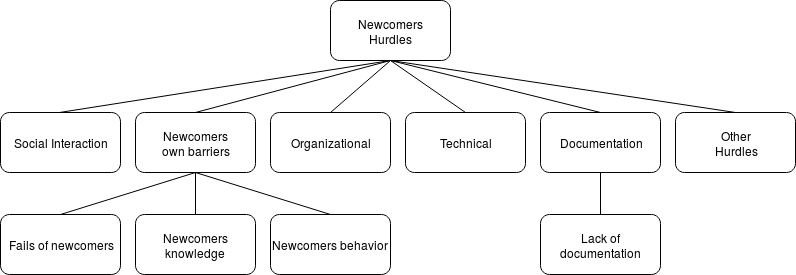
\includegraphics[scale=0.65]{BarriersCategorized.png}
	\caption{Categories of newcomers hurdles}
	\label{img:hurdles_categories}
\end{figure*}

\section{Support newcomer to overcome the barriers's}
\begin{itemize}
\item Crowdsourcing in SE -\cite{LaToza2016}
\item On the Relationship between Newcomer Motivations and Contribution Barriers Open Source Projects -\cite{Hannebauer2017}
\item Barriers faced by newcomers to software crowdsourcing projects -\cite{Zanatta2017}
\item Beyond pretty pictures: Examining the benefits of code visualization for Open Source newcomers\cite{Park2009}
	\subitem "results show that visualization tools made it easier for participants to find information by presenting large amounts of 						data in an accessible form."
\item Increasing the Self-Efficacy of Newcomers to Open Source Software Projects\cite{Steinmacher2015}
\item Patterns for tearing down contribution barriers to FLOSS projects\cite{Wolff-Marting2013}
\end{itemize} 


\section{conclusion and future work}
Sort the barriers and motivations and further investigate those (Es ist eine ansammlung die noch nicht unterteilt ist)




% Literaturverzeichnis
\printbibliography



\end{document}